\documentclass[conference]{IEEEtran}
\usepackage[utf8]{inputenc}
\usepackage{amsmath}
\usepackage{amsfonts}
\usepackage{amssymb}
\usepackage{graphicx}
\usepackage[colorlinks=false, hidelinks=false, urlcolor=black]{hyperref}
\usepackage{float}
\usepackage{subcaption}
\usepackage{cite}


\title{Aplicación de la Transformada Rápida de Fourier en el Filtrado de Imágenes en el Dominio de Frecuencias}

\author{
\IEEEauthorblockN{D. R. Argueta Bran}
\IEEEauthorblockA{\textit{Universidad Centroamericana Jose simeon cañas}\\
\texttt{00042220@uca.edu.sv}
}
\and
\IEEEauthorblockN{A. G. Merlos Rodríguez}
\IEEEauthorblockA{\textit{Universidad Centroamericana Jose simeon cañas}\\
\texttt{00005118@uca.edu.sv}
}
\and
\IEEEauthorblockN{\hspace{2cm}K. E. Rodas Escobar}
\IEEEauthorblockA{\hspace{2cm}\textit{Universidad Centroamericana Jose simeon cañas}\\
\texttt{\hspace{2cm}00226013@uca.edu.sv}
}
\and
\IEEEauthorblockN{\hspace{1.5cm}I. M. Huezo Beltrán}
\IEEEauthorblockA{\hspace{1.5cm}\textit{Universidad Centroamericana Jose simeon cañas}\\
\texttt{\hspace{1.5cm}00233121@uca.edu.sv}
}
\and
\IEEEauthorblockN{\hspace{1.8cm}R. F. Rivas Díaz}
\IEEEauthorblockA{\hspace{1.8cm}\textit{Universidad Centroamericana Jose simeon cañas}\\
\texttt{\hspace{1.8cm}00131321@uca.edu.sv}
}
}

\begin{document}

\maketitle

\renewcommand{\abstractname}{Resumen}
\begin{abstract}
El procesamiento de imágenes mediante la Transformada Rápida de Fourier (FFT) es una técnica fundamental en el análisis y manipulación de señales bidimensionales. Este trabajo presenta un estudio teórico-práctico de la aplicación de la FFT para el filtrado de imágenes en el dominio de frecuencias. Se abordan los fundamentos matemáticos de la Transformada Discreta de Fourier (DFT) bidimensional, su optimización mediante la FFT, y su aplicación en la eliminación de ruido periódico, suavizado mediante filtros pasa-bajos y detección de bordes con filtros pasa-altos. Los experimentos realizados demuestran la efectividad del filtrado en frecuencia para tareas de mejora y restauración de imágenes.
\end{abstract}

\section{Introducción}

El análisis de Fourier, desde su formulación original por Jean-Baptiste Joseph Fourier en el siglo XIX, ha revolucionado múltiples campos de la ciencia y la ingeniería. La idea fundamental de descomponer una señal compleja en sus componentes senoidales elementales ha permitido abordar problemas que de otra forma serían intratables en el dominio temporal o espacial.

En el contexto del procesamiento digital de imágenes, la Transformada Discreta de Fourier (DFT) y su implementación eficiente, la Transformada Rápida de Fourier (FFT), constituyen herramientas indispensables. La DFT permite transformar una imagen del dominio espacial al dominio de frecuencias, donde las operaciones de filtrado, compresión y análisis espectral se vuelven computacionalmente más eficientes y conceptualmente más claras \cite{berkeley2024}.

El presente trabajo se enfoca en la aplicación de la FFT para el filtrado de imágenes en el dominio de frecuencias. Específicamente, se aborda:
\begin{itemize}
    \item La eliminación de ruido periódico mediante filtros de rechazo de banda.
    \item El suavizado de imágenes a través de filtros pasa-bajos.
    \item La detección de bordes utilizando filtros pasa-altos.
\end{itemize}

El objetivo es proporcionar una comprensión teórica y práctica de estas técnicas, demostrando su efectividad a través de experimentos implementados en Python utilizando la biblioteca NumPy \cite{numpy2024}.

\section{Marco Teórico}

\subsection{Transformada Discreta de Fourier (DFT)}

La Transformada Discreta de Fourier es una herramienta matemática que transforma una secuencia de $N$ números complejos $x[n]$ en otra secuencia $X[k]$ de igual longitud, representando las componentes de frecuencia de la señal original. Para el caso unidimensional, la DFT se define como:

\begin{equation}
X[k] = \sum_{n=0}^{N-1} x[n] e^{-j2\pi kn/N}, \quad k = 0, 1, \ldots, N-1
\label{eq:dft1d}
\end{equation}

donde $j = \sqrt{-1}$ es la unidad imaginaria y $N$ es el número de muestras \cite{kulkarni2019}.

La transformada inversa permite reconstruir la señal original a partir de sus componentes espectrales:

\begin{equation}
x[n] = \frac{1}{N} \sum_{k=0}^{N-1} X[k] e^{j2\pi kn/N}, \quad n = 0, 1, \ldots, N-1
\label{eq:idft1d}
\end{equation}

\subsection{Transformada Discreta de Fourier Bidimensional}

Para el procesamiento de imágenes, se extiende la DFT a dos dimensiones. Dada una imagen de tamaño $M \times N$ representada como $f(x,y)$, la DFT bidimensional se define como:

\begin{equation}
F(u,v) = \sum_{x=0}^{M-1} \sum_{y=0}^{N-1} f(x,y) e^{-j2\pi(ux/M + vy/N)}
\label{eq:dft2d}
\end{equation}

donde $F(u,v)$ es la representación en el dominio de frecuencias, con $u = 0, 1, \ldots, M-1$ y $v = 0, 1, \ldots, N-1$ \cite{gonzalez2018}.

La transformada inversa correspondiente es:

\begin{equation}
f(x,y) = \frac{1}{MN} \sum_{u=0}^{M-1} \sum_{v=0}^{N-1} F(u,v) e^{j2\pi(ux/M + vy/N)}
\label{eq:idft2d}
\end{equation}

\subsection{Propiedades de la DFT}

\subsubsection{Separabilidad}

La DFT bidimensional es separable, lo que significa que puede calcularse aplicando la DFT unidimensional primero a las filas y luego a las columnas:

\begin{equation}
F(u,v) = \sum_{x=0}^{M-1} e^{-j2\pi ux/M} \sum_{y=0}^{N-1} f(x,y) e^{-j2\pi vy/N}
\label{eq:separabilidad}
\end{equation}

Esta propiedad es fundamental para la implementación eficiente de la FFT 2D \cite{groningen2024}.

\subsubsection{Simetría Conjugada}

Para imágenes reales, la DFT presenta simetría conjugada:

\begin{equation}
F(u,v) = F^*(-u,-v)
\label{eq:simetria}
\end{equation}

donde $F^*$ denota el conjugado complejo. Esta propiedad implica que el espectro de magnitud es simétrico con respecto al origen \cite{smith2003}.

\subsubsection{Teorema de Convolución}

El teorema de convolución establece que la convolución en el dominio espacial equivale a la multiplicación en el dominio de frecuencias:

\begin{equation}
\mathcal{F}\{f(x,y) * h(x,y)\} = F(u,v) \cdot H(u,v)
\label{eq:convolucion}
\end{equation}

donde $*$ denota convolución y $\mathcal{F}$ es la transformada de Fourier \cite{gockenbach2010}. Esta propiedad es la base del filtrado en frecuencia, ya que permite aplicar filtros simplemente multiplicando el espectro de la imagen por una función de transferencia.

\subsection{Transformada Rápida de Fourier (FFT)}

La Transformada Rápida de Fourier es un algoritmo eficiente para calcular la DFT. Su desarrollo se atribuye a Cooley y Tukey en 1965, aunque existen trabajos previos de Gauss \cite{cooley1967}.

El algoritmo de Cooley-Tukey se basa en el paradigma de divide y conquista. Para $N = 2^m$, descompone la DFT de tamaño $N$ en dos DFT de tamaño $N/2$:

\begin{equation}
\begin{split}
X[k] &= \sum_{n=0}^{N/2-1} x[2n] \, e^{-j2\pi kn/(N/2)} \\ 
     &+ \, e^{-j2\pi k/N} \sum_{n=0}^{N/2-1} x[2n+1] \, e^{-j2\pi kn/(N/2)}
\end{split}
\label{eq:cooley}
\end{equation}

Esta descomposición reduce la complejidad computacional de $\mathcal{O}(N^2)$ a $\mathcal{O}(N \log N)$, lo que hace factible el procesamiento de imágenes de gran tamaño en tiempo real \cite{johnson2020}.

Para el caso bidimensional, la FFT se aplica de manera separable, realizando primero la FFT 1D a cada fila y luego a cada columna \cite{numpy2024}.

\subsection{Filtrado en el Dominio de Frecuencias}

El filtrado en el dominio de frecuencias consiste en modificar selectivamente las componentes espectrales de una imagen. Este proceso se realiza siguiendo los siguientes pasos:

\begin{enumerate}
    \item Calcular la DFT de la imagen: $F(u,v) = \mathcal{F}\{f(x,y)\}$
    \item Aplicar un filtro: $G(u,v) = H(u,v) \cdot F(u,v)$
    \item Calcular la transformada inversa: $g(x,y) = \mathcal{F}^{-1}\{G(u,v)\}$
\end{enumerate}

donde $H(u,v)$ es la función de transferencia del filtro \cite{berkeley2024}.

\subsubsection{Filtro Pasa-Bajos Ideal}

Un filtro pasa-bajos ideal elimina las altas frecuencias y conserva las bajas. Su función de transferencia es:

\begin{equation}
H(u,v) = 
\begin{cases}
1 & \text{si } \sqrt{u^2 + v^2} \leq D_0 \\
0 & \text{si } \sqrt{u^2 + v^2} > D_0
\end{cases}
\label{eq:pasa_bajos}
\end{equation}

donde $D_0$ es el radio de corte. Este filtro produce suavizado y elimina ruido de alta frecuencia, pero puede introducir artefactos de Gibbs en los bordes \cite{gonzalez2018}.

\subsubsection{Filtro Pasa-Altos Ideal}

El filtro pasa-altos es complementario al pasa-bajos, eliminando las bajas frecuencias y conservando las altas:

\begin{equation}
H(u,v) = 
\begin{cases}
0 & \text{si } \sqrt{u^2 + v^2} \leq D_0 \\
1 & \text{si } \sqrt{u^2 + v^2} > D_0
\end{cases}
\label{eq:pasa_altos}
\end{equation}

Este filtro resalta bordes y detalles finos \cite{smith2003}.

\subsubsection{Filtro Gaussiano}

Para evitar los artefactos producidos por los filtros ideales, se utilizan filtros con transiciones suaves. El filtro Gaussiano tiene una función de transferencia:

\begin{equation}
H(u,v) = e^{-(u^2 + v^2) / (2\sigma^2)}
\label{eq:gaussiano}
\end{equation}

donde $\sigma$ controla el ancho de la banda. Este filtro produce un suavizado sin artefactos de Gibbs \cite{szeliski2010}.

\subsubsection{Rechazo de Ruido Periódico}

El ruido periódico se manifiesta en el dominio de frecuencias como picos aislados en posiciones específicas. Para eliminarlo, se emplean filtros de rechazo de banda:

\begin{equation}
H(u,v) = 
\begin{cases}
0 & \text{si } \sqrt{(u-u_0)^2 + (v-v_0)^2} \leq W \\
1 & \text{en otro caso}
\end{cases}
\label{eq:rechazo_banda}
\end{equation}

donde $(u_0, v_0)$ son las coordenadas del pico de ruido y $W$ es el ancho de la banda de rechazo \cite{gonzalez2018}.

\subsection{Teoremas Relevantes}

\subsubsection{Teorema de Parseval}

El teorema de Parseval establece la conservación de la energía en la transformada de Fourier:

\begin{equation}
\sum_{x=0}^{M-1} \sum_{y=0}^{N-1} |f(x,y)|^2 = \frac{1}{MN} \sum_{u=0}^{M-1} \sum_{v=0}^{N-1} |F(u,v)|^2
\label{eq:parseval}
\end{equation}

Este teorema es fundamental para el análisis de la energía de la señal en ambos dominios \cite{gockenbach2010}.

\subsubsection{Teorema de Muestreo (Nyquist)}

El teorema de Nyquist establece que para reconstruir correctamente una señal, la frecuencia de muestreo debe ser al menos el doble de la frecuencia máxima presente en la señal \cite{smith2003}. En el contexto de imágenes, esto implica que los detalles finos (altas frecuencias) requieren una resolución espacial adecuada.

\section{Metodología}

\subsection{Herramientas Computacionales}

Para la implementación experimental se utilizaron las siguientes herramientas:

\begin{itemize}
    \item \textbf{Python 3.8+}: Lenguaje de programación para la implementación.
    \item \textbf{NumPy}: Biblioteca para computación numérica y operaciones con arrays.
    \item \textbf{Matplotlib}: Biblioteca para visualización de resultados.
    \item \textbf{Scikit-image}: Biblioteca para procesamiento de imágenes.
    \item \textbf{SciPy}: Biblioteca para operaciones científicas avanzadas.
\end{itemize}

\subsection{Obtención de Imágenes}

Se utilizaron dos tipos de imágenes:
\begin{enumerate}
    \item \textbf{Imagen de prueba}: Imagenes de internet de diversas resoluciones, desde 144p a 4K.
    \item \textbf{Imagen con ruido periódico}: Generada sintéticamente agregando una señal senoidal 2D a la imagen original:
    
    \begin{equation}
\begin{split}
f_{ruidosa}(x,y) &= f_{original}(x,y) \\
                 &+ A \sin(2\pi f_x x/M) \sin(2\pi f_y y/N)
\end{split}
\label{eq:ruido_periodico}
\end{equation}
\end{enumerate}

\subsection{Procedimiento Experimental}

Se realizaron cuatro experimentos principales:

\subsubsection{Experimento 1: Visualización del Espectro de Frecuencias}

Para cada imagen, se calculó la FFT bidimensional utilizando la función \texttt{np.fft.fft2()}, seguida de un desplazamiento con \texttt{np.fft.fftshift()} para centrar las bajas frecuencias. Se visualizó el espectro de magnitud en escala logarítmica:

\begin{equation}
S(u,v) = \log(1 + |F(u,v)|)
\label{eq:espectro}
\end{equation}

\subsubsection{Experimento 2: Filtrado Pasa-Bajos}

Se aplicó un filtro pasa-bajos ideal con radio $D_0 = 30$ píxeles. La imagen filtrada se obtuvo mediante la transformada inversa de $G(u,v) = H_{PB}(u,v) \cdot F(u,v)$.

\subsubsection{Experimento 3: Filtrado Pasa-Altos}

Se aplicó un filtro pasa-altos ideal con radio $D_0 = 20$ píxeles. Se visualizó el resultado normalizado para resaltar los bordes.

\subsubsection{Experimento 4: Eliminación de Ruido Periódico}

Se identificaron los picos en el espectro de la imagen ruidosa y se aplicó un filtro de rechazo de banda con radio $W = 5$ píxeles alrededor de cada pico.
\hfill
\hfill
\section{Resultados}

\subsection{Espectro de Frecuencias}

La Figura 1 muestra el espectro de frecuencias de la imagen original y de la imagen con ruido periódico. En el espectro de la imagen ruidosa se observan claramente cuatro picos aislados correspondientes a las componentes del ruido senoidal, ubicados simétricamente con respecto al centro.

\begin{figure}[H]
    \centering
    \begin{subfigure}{0.3\textwidth}
        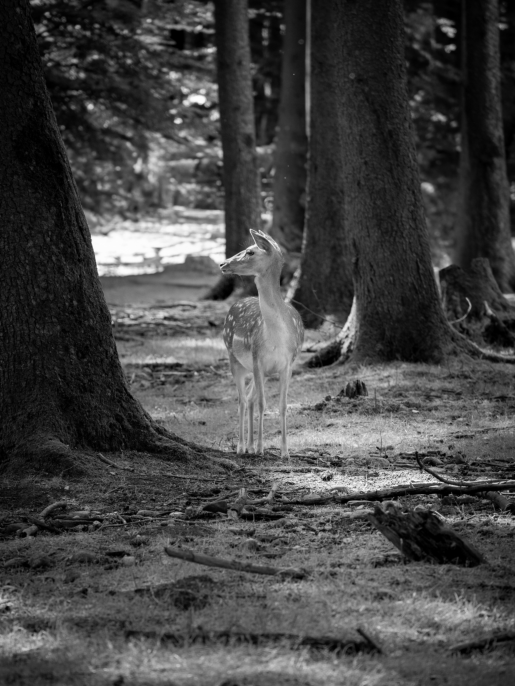
\includegraphics[width=\textwidth]{figuras/image-original.PNG}
        \caption{Espectro de la imagen original}
        \label{fig:espectro_original}
    \end{subfigure}
    \hfill
    \begin{subfigure}{0.3\textwidth}
        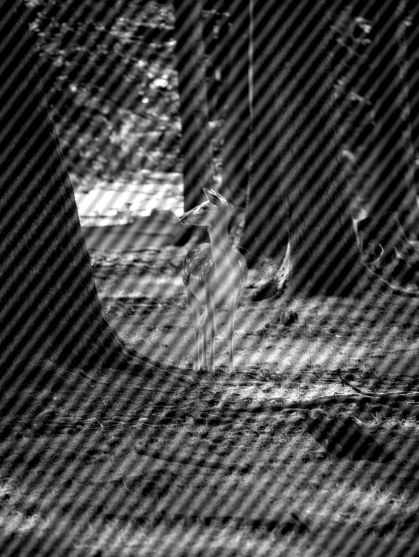
\includegraphics[width=\textwidth]{figuras/image-con-ruido-periodico.PNG}
        \caption{Espectro de la imagen con ruido}
        \label{fig:espectro_ruidoso}
    \end{subfigure}
    \caption{Espectro de frecuencias en escala logarítmica}
    \label{fig:espectros}
\end{figure}
\newpage
\subsection{Filtro Pasa-Bajos}

La Figura 2 muestra el efecto del filtro pasa-bajos. La imagen resultante presenta un suavizado notable, eliminando detalles finos y ruido de alta frecuencia. Se observa una pérdida de nitidez en bordes y texturas.

\begin{figure}[H]
    \centering
    \begin{subfigure}{0.3\textwidth}
    \centering
        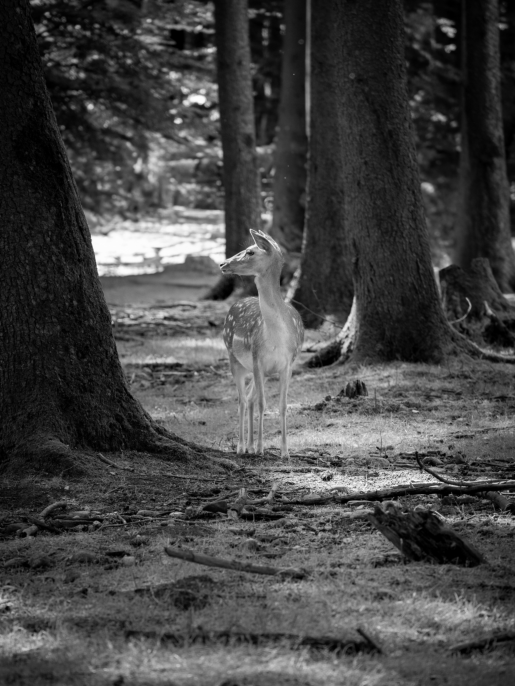
\includegraphics[width=0.85\textwidth]{figuras/image-original.PNG}
        \caption{Original}
        \label{fig:original}
    \end{subfigure}
    \hfill
    \begin{subfigure}{0.3\textwidth}
    \centering
        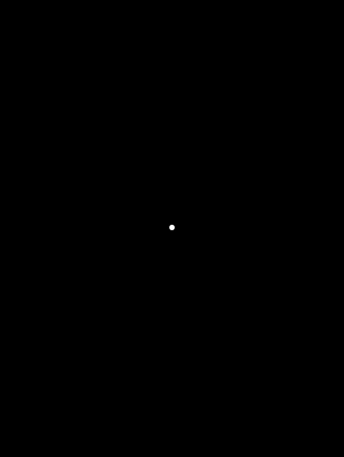
\includegraphics[width=0.85\textwidth]{figuras/image-mascara-pasa-bajos.PNG}
        \caption{Máscara pasa-bajos}
        \label{fig:mascara_pb}
    \end{subfigure}
    \hfill
    \begin{subfigure}{0.3\textwidth}
    \centering
        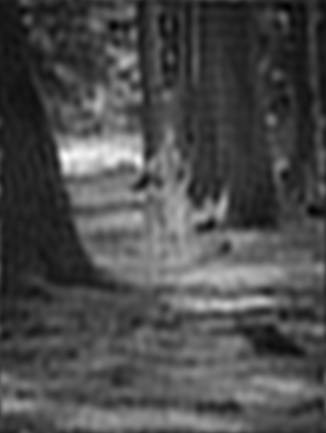
\includegraphics[width=0.85\textwidth]{figuras/image-filtrada-pasa-bajos.PNG}
        \caption{Imagen filtrada}
        \label{fig:pasa_bajos}
    \end{subfigure}
    \caption{Efecto del filtro pasa-bajos ($D_0 = 30$)}
    \label{fig:resultado_pb}
\end{figure}


\subsection{Filtro Pasa-Altos}


El filtro pasa-altos (Figura 3) resalta las transiciones bruscas de intensidad, correspondientes a bordes y detalles finos. La imagen resultante, visualizada en valores absolutos normalizados, muestra claramente los contornos de la imagen original.
\hfill

\begin{figure}[H]
    \centering
    \begin{subfigure}{0.3\textwidth}
    \centering
        
\includegraphics[width=0.85\textwidth]{figuras/image-mascara-pasa-altos.PNG}
        \caption{Máscara pasa-altos}
        \label{fig:mascara_pa}
    \end{subfigure}
    \hfill
    \begin{subfigure}{0.3\textwidth}
    \centering
        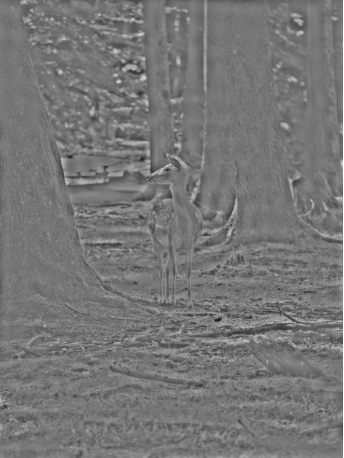
\includegraphics[width=0.85\textwidth]{figuras/image-filtrada-pasa-altos-bordes.PNG}
        \caption{Imagen filtrada}
        \label{fig:pasa_altos}
    \end{subfigure}
    \hfill
    \begin{subfigure}{0.3\textwidth}
    \centering
        
\includegraphics[width=0.85\textwidth]{figuras/bordes-detectados-umbralizado.PNG}
        \caption{Bordes umbralizados}
        \label{fig:bordes}
    \end{subfigure}
    \caption{Efecto del filtro pasa-altos ($D_0 = 20$)}
    \label{fig:resultado_pa}
\end{figure}
\hfill
\subsection{Eliminación de Ruido Periódico}

La Figura 4 muestra el proceso de eliminación de ruido periódico. Se observa que la máscara de rechazo elimina efectivamente los picos en el espectro, resultando en una imagen significativamente más limpia.

\begin{figure}[H]
    \centering
    \begin{subfigure}{0.22\textwidth}
        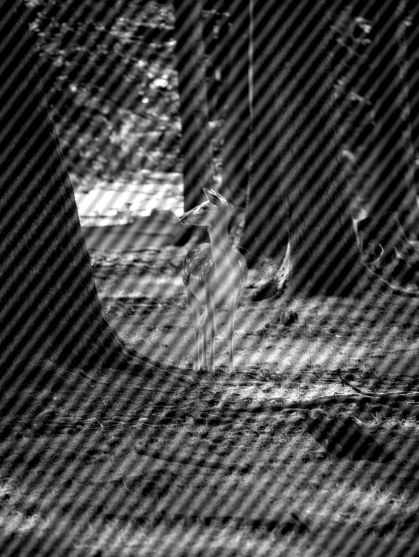
\includegraphics[width=\textwidth]{figuras/image-con-ruido-periodico.PNG}
        \caption{Imagen ruidosa}
        \label{fig:ruidosa}
    \end{subfigure}
    \hfill
    \begin{subfigure}{0.22\textwidth}
        
\includegraphics[width=\textwidth]{figuras/image-mascara-de-rechazo.PNG}
        \caption{Máscara rechazo}
        \label{fig:mascara_rechazo}
    \end{subfigure}
    \hfill
    \begin{subfigure}{0.22\textwidth}
        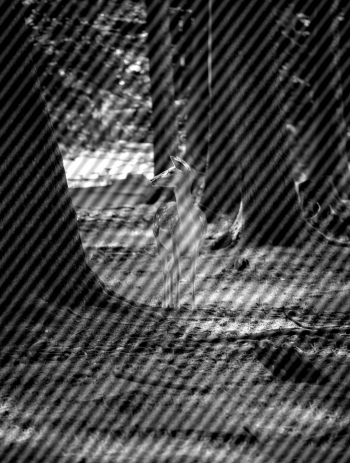
\includegraphics[width=\textwidth]{figuras/image-sin-ruido.PNG}
        \caption{Imagen sin ruido}
        \label{fig:denoised}
    \end{subfigure}
    \hfill
    \begin{subfigure}{0.22\textwidth}
        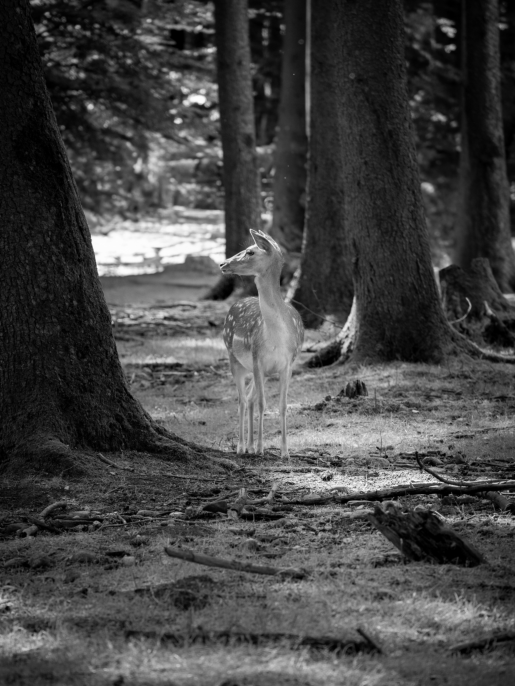
\includegraphics[width=\textwidth]{figuras/image-original.PNG}
        \caption{Original (referencia)}
        \label{fig:referencia}
    \end{subfigure}
    \caption{Eliminación de ruido periódico}
    \label{fig:resultado_rechazo}
\end{figure}

\subsection{Análisis de Resultados}

Los experimentos realizados demuestran la efectividad del filtrado en el dominio de frecuencias:

\begin{itemize}
    \item El \textbf{filtro pasa-bajos} elimina eficazmente el ruido de alta frecuencia, aunque produce una pérdida de detalles finos. El efecto de suavizado es comparable al de un filtro de mediana en el dominio espacial \cite{szeliski2010}.
    
    \item El \textbf{filtro pasa-altos} resalta bordes y transiciones, siendo útil para tareas de detección de bordes y realce de detalles. La umbralización de la imagen filtrada permite aislar las estructuras principales.
    
    \item La \textbf{eliminación de ruido periódico} demuestra ser extremadamente efectiva, ya que el ruido se concentra en picos aislados en el espectro. Este método es superior a cualquier filtro espacial para este tipo específico de ruido \cite{gonzalez2018}.
    
    \item Los \textbf{filtros ideales} (pasa-bajos y pasa-altos) presentan artefactos de Gibbs en las transiciones. Los filtros Gaussianos o Butterworth ofrecen una alternativa con transiciones más suaves y menos artefactos \cite{johnson2020}.
\end{itemize}

\section{Conclusiones}

En este trabajo se ha presentado un estudio teórico-práctico de la aplicación de la Transformada Rápida de Fourier en el filtrado de imágenes en el dominio de frecuencias. Los principales hallazgos y conclusiones son:

\begin{enumerate}
    \item La DFT bidimensional constituye una herramienta fundamental para el análisis espectral de imágenes, permitiendo identificar y modificar selectivamente componentes de frecuencia específicas.
    
    \item La FFT, mediante su implementación eficiente basada en el algoritmo de Cooley-Tukey, hace factible el procesamiento de imágenes en tiempo real al reducir la complejidad computacional de $\mathcal{O}(N^2)$ a $\mathcal{O}(N \log N)$.
    
    \item El filtrado en el dominio de frecuencias ofrece ventajas significativas para:
    \begin{itemize}
        \item Eliminación de ruido periódico (superior a métodos espaciales).
        \item Filtrado selectivo de bandas de frecuencia.
        \item Operaciones de suavizado y realce con control preciso.
    \end{itemize}
    
    \item La elección del tipo de filtro depende de la aplicación específica:
    \begin{itemize}
        \item Filtros ideales: simples pero con artefactos de Gibbs.
        \item Filtros Gaussianos/Butterworth: transiciones suaves, menos artefactos.
        \item Filtros de rechazo de banda: ideales para ruido periódico.
    \end{itemize}
    
    \item El filtrado en frecuencia, aunque poderoso, presenta limitaciones:
    \begin{itemize}
        \item Puede introducir artefactos en los bordes debido al truncamiento de frecuencias.
        \item Requiere conversión a escala de grises para imágenes a color (aunque puede extenderse a cada canal RGB).
        \item La identificación manual de picos de ruido puede ser laboriosa para imágenes con patrones complejos.
    \end{itemize}
\end{enumerate}

\subsection{Trabajo Futuro}

Como líneas de investigación futura se sugieren:
\begin{itemize}
    \item Implementación de detección automática de picos de ruido periódico.
    \item Extensión del método a imágenes a color mediante procesamiento en cada canal RGB.
    \item Aplicación de la FFT para compresión de imágenes (similar al estándar JPEG que utiliza DCT).
    \item Comparación cuantitativa de diferentes tipos de filtros utilizando métricas como PSNR (Peak Signal-to-Noise Ratio) y SSIM (Structural Similarity Index).
\end{itemize}

\begin{thebibliography}{99}

\bibitem{berkeley2024}
Python Numerical Methods at Berkeley, "Discrete Fourier Transform," 2024. [Online]. Available: \url{https://pythonnumericalmethods.studentorg.berkeley.edu/notebooks/chapter24.02-Discrete-Fourier-Transform.html}

\bibitem{numpy2024}
NumPy, "numpy.fft.fft," NumPy v2.2 Manual, 2024. [Online]. Available: https://numpy.org/doc/2.2/reference/generated/numpy.fft.fft.html

\bibitem{kulkarni2019}
S. R. Kulkarni, "Frequency Domain and Fourier Transforms," Princeton University, 2019. [Online]. Available:
\url{https://www.princeton.edu/~cuff/ele201/kulkarni_text/frequency.pdf}

\bibitem{gonzalez2018}
R. C. Gonzalez and R. E. Woods, \textit{Digital Image Processing}, 4th ed. Pearson, 2018.

\bibitem{groningen2024}
University of Groningen, "Fourier Transforms Notebook," 2024. [Online]. Available: 
\url{https://www.astro.rug.nl/intranet/courses/PROGNUMNEW/latest/build/html/Notebooks/fourierTransforms.html}

\bibitem{smith2003}
S. W. Smith, \textit{Digital Signal Processing: A Practical Guide for Engineers and Scientists}. Newnes, 2003.

\bibitem{gockenbach2010}
M. S. Gockenbach, \textit{Applied Computational Linear Algebra}. SIAM, 2010.

\bibitem{cooley1967}
J. W. Cooley, P. A. W. Lewis, and P. W. Welch, "Historical notes on the fast Fourier transform," \textit{Proceedings of the IEEE}, vol. 55, no. 10, pp. 1675-1677, 1967.

\bibitem{johnson2020}
S. G. Johnson, "Notes on FFT Derivation," MIT, 2011. [Online]. Available:
\url{https://math.mit.edu/~stevenj/fft-deriv.pdf}

\bibitem{szeliski2010}
R. Szeliski, \textit{Computer Vision: Algorithms and Applications}. Springer, 2010.

\bibitem{peyre2024}
G. Peyré, "Numerical Tours in Python - Fourier Processing," 2024. [Online]. Available: 
\url {https://nbviewer.org/github/gpeyre/numerical-tours/blob/master/python/}

\end{thebibliography}

\end{document}